\documentclass[11pt,letterpaper]{article}
\usepackage[lmargin=1in,rmargin=1in,tmargin=1in,bmargin=1in]{geometry}
\usepackage{../style/homework}
\usepackage{../style/commands}
\setbool{quotetype}{false} % True: Side; False: Under
\setbool{hideans}{false} % Student: True; Instructor: False

% -------------------
% Content
% -------------------
\begin{document}

\homework{3: Due 09/28}{This year I'm lovin’ someone who deserves me. Me.}{Suzanne `Crazy Eyes' Warren, Orange is the New Black}

% Problem 1
\problem{10} Let $C(x)$ be the cost function given by $C(x):= 3.50x + 15$.
\begin{enumerate}[(a)]
\item Find the total cost in producing 100 items. \pspace
	\[
	C(100)= 3.50(100) + 15= 350 + 15= 365
	\] \pvspace{1.3cm}

\item If the company makes 100 items, what is the average cost of production per item? \pspace
	\[
	\dfrac{C(100)}{100}= \dfrac{365}{100}= 3.65
	\] \pvspace{1.1cm}

\item What is the production cost per item? \pvspace{1.2cm}

{\itshape Because the function is linear, this is the slope of the cost function, which is 3.50.} \pvspace{1.3cm}

\item Find the $y$-intercept for $C(x)$. \pspace
	\[
	C(0)= 3.50(0) + 15= 0 + 15= 15
	\]
{\itshape Therefore, the $y$-intercept is $(0, 15)$.} \pvspace{0.8cm}

\item Interpret your answer from (d). \pspace

{\itshape The $y$-intercept occurs when $x= 0$, i.e. when we produce 0 items. But then any cost associated with producing nothing must be the fixed costs.}
\end{enumerate}



\newpage



% Problem 2
\problem{10} Let $R(x)$ be the revenue function given by $R(x):= 15.99x$. 
\begin{enumerate}[(a)]
\item What is the price per item that the company sets? \pspace

{\itshape Because the revenue function is a linear function, the price per item is the slope of the line, which is 15.99.}
	\[
	\$15.99
	\] \pvspace{4.3cm}

\item How much revenue is gained by selling 150 items? \pspace
	\[
	R(150)= 15.99(150)= \$2398.50
	\] \pvspace{4.7cm}

\item How many items would the company need to sell to make at least \$2,000 in revenue? 
	\[
	\begin{aligned}
	R(x)&= 2000 \\
	15.99x&= 2000 \\
	x&= 125.078
	\end{aligned}
	\]
{\itshape The company cannot sell 125.078 items (presumably). Then the must sell either 125 or 126 items. Selling less would result in less revenue. Therefore, the company needs to sell at least 126 items.}
\end{enumerate}



\newpage



% Problem 3
\problem{10} Let the revenue and cost functions for a company be given by $R(x):= 24.99x$ and $C(x)= 11.20x + 560$. 
\begin{enumerate}[(a)]
\item Find the profit function, $P(x)$. \pspace
	\[
	P(x)= R(x) - C(x)= 24.99x - (11.20x + 560) = 24.99x - 11.20x - 560= 13.79x - 560
	\] \pvspace{2.2cm}

\item Find the breakeven point. \pspace
	\[
	\begin{aligned}
	P(x)&= 0 \\
	13.79x - 560&= 0 \\
	13.79x&= 560 \\
	x&= 40.609
	\end{aligned}
	\] \pvspace{1.2cm}

\item What does the breakeven point represent on the graph of $P(x)$? \pspace

{\itshape The breakeven point is the point where profit is 0. But then $P(x)= 0$. Then this must be a $x$-intercept for $P(x)$.} \pvspace{3cm}

\item Sketch the functions $R(x), C(x)$ and $P(x)$ along with the breakeven point. \pspace
	\[
	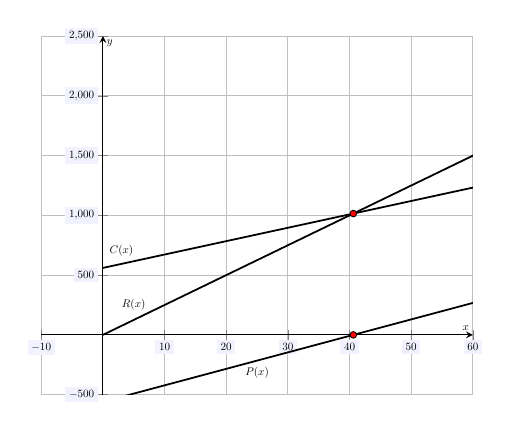
\begin{tikzpicture}[scale=0.8,every node/.style={scale=0.5}]
	\begin{axis}[
	grid=both,
	axis lines=middle,
	ticklabel style={fill=blue!5!white},
	xmin= -10, xmax=60,
	ymin= -500, ymax=2500,
	xtick={-10,0,...,60},
	ytick={-500,0,...,5000},
	xlabel=\(x\),ylabel=\(y\),
	]
	\addplot[thick, domain= 0:100] {24.99*x};
	\addplot[thick, domain= 0:100] {11.20*x + 560};
	\addplot[thick, domain= 0:100] {13.79*x - 560};
	\node at (3,700) {$C(x)$};
	\node at (5,250) {$R(x)$};
	\node at (25,-320) {$P(x)$};
	
	\draw[fill=red] (40.609,1014.82) circle (1.5pt);
	\draw[fill=red] (40.609,0) circle (1.5pt);
	\end{axis}
	\end{tikzpicture}
	\]
\end{enumerate}



\newpage



% Problem 4
\problem{10} A fine dining restaurant orders high-quality salmon for their menu. When bought in bulk, each salmon costs \$11.99 and there is a flat delivery fee of \$210. To turn profit on the fish orders, the restaurant marks the price up by 80\%. What is the smallest number of salmon they have to order and sell to make a profit on their salmon sales? \pspace

\sol {\itshape First, we find the revenue function. We know that the salmon costs \$11.99. The restaurant will mark this up by 80\%. Therefore, the price of the salmon will be $\$11.99(1.8)= \$21.582$. Then the revenue function is $R(x)= 21.582x$. \pspace

Now we need to find the cost function. We know they are charged a delivery of \$210---the fixed cost. Each salmon costs \$11.99, so the variable cost is $11.99x$. Therefore, the (total) cost function is $C(x)= 11.99x + 210$. \pspace

To find the point at which they start to turn a profit on salmon sales, we need to find the breakeven point. We can do this either by finding when $R(x)= C(x)$, or we can find the profit function, $P(x)$, and then find when $P(x)= 0$. We choose the latter. We know $P(x)= R(x) - C(x)$. But then
	\[
	P(x)= R(x) - C(x)= 21.582x - (11.99x + 210)= 21.582x - 11.99x - 210= 9.592x - 210
	\]
Now we find when $P(x)= 0$:
	\[
	\begin{aligned}
	P(x)&= 0 \\
	9.592x - 210&= 0 \\
	9.592x&= 210 \\
	x&= 21.89
	\end{aligned}
	\]
Because the restaurant cannot sell $21.89$ salmon, they must sell either 21 or 22 to break even. However, selling less fish clearly makes less money and $x= 21.89$ is the exact point where they break even, they must sell at least 22 salmon.}


\end{document}